\section{Scaling Performance of $256^{3}$ problem}
Many authors in past have highlighted how bigger problems provide better scaling capabilities and our $256^{3}$ simulation fulfill such trend.
The medium sized problem shows better scaling performances compared to the small ones, although exhibit a slightly rugged behavior.
\par
\begin{figure}
\begin{center}
\includegraphics[scale=0.6]{grafici/1281}
\caption{Scaling performance of $256^{3}$ simulation}
\label{1281}
\end{center}
\end{figure}

\begin{figure}
\begin{center}
\includegraphics[scale=0.6]{grafici/1283}
\caption{Efficiency factor of $256^{3}$ simulation}
\label{1283}
\end{center}
\end{figure}

A slab decomposed algorithm provide gains of $\mathcal{O}(10)$ in terms of execution times, less than a pencil decomposed algorithm, but with better results for small processors grid. In fact, as depicted in figure~\ref{1281} the 1D decomposition curve achieve lower execution times than the 2D ones, until 32 cores.\\
Passed 32 cores the pencil decomposition prevails, reaching speedup factors above 120, with time savings in the order of magnitude of $\mathcal{O}(100)$ with respect to the single core runtime.
In the figure~\ref{1283} is possible to see the efficiencies achieved by the two methods, running on 64 threads per processor. It is important to denote the behavior of the pencil decomposed algorithm, which, until 8 cores in use, exhibits a very high scaling efficiency. \\
\par
Comparing image~\ref{1281} with its counterpart for the $128^{3}$ problem, figure~\ref{641} of page~\pageref{641}, we can see that the curves are quite similar. Both exhibits a very good fitting with the theoretical ones until 16 parallel processes take place. Once passed this threshold, the bigger problem maintains a better scaling efficiency, as we could see by comparing figure~\ref{1283} and~\ref{643}, for both decomposition methods. \par
The better efficiency allows to reach higher speedup factors at number of processes equality, and the larger dimensions move the performances peak towards higher number of threads, as is possible to see by looking at figure~\ref{1282}. The combination of this two factors doubles the last speedup factor, passing from 57, for the $128^{3}$ problem, to 122 for the $256^{3}$.\\

\begin{figure}
\begin{center}
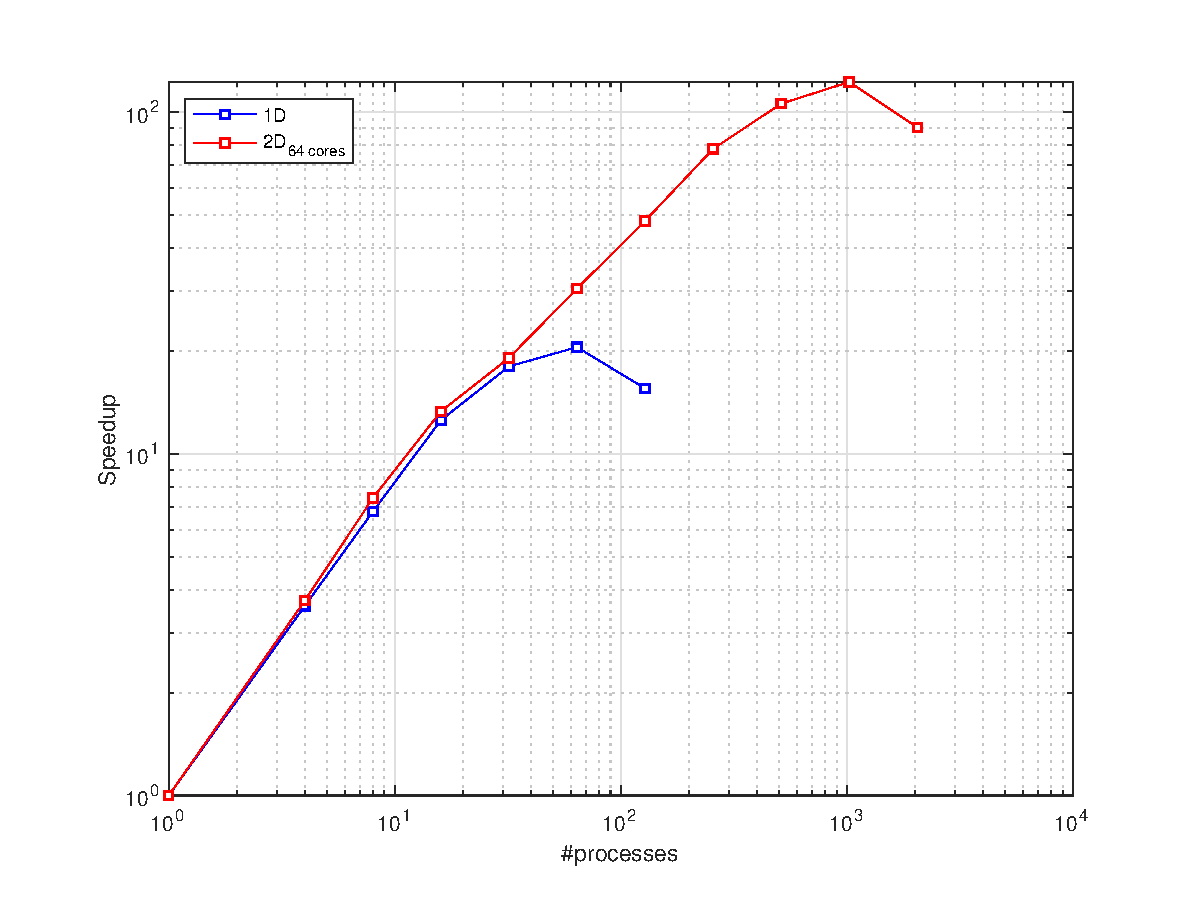
\includegraphics[scale=0.6]{grafici/1282}
\caption{Speedup performance factor of $256^{3}$ simulation}
\label{1282}
\end{center}
\end{figure}

\par
A comparison of the performances of 1D decomposition against the 2D for the present problem dimension is presented in table~\ref{128:data} of page~\pageref{128:data}.

\begin{table}
\caption{Data from $256^{3}$ simulation}
\begin{center}
\begin{tabular}{c c c c c}
\toprule
\textbf{\#Processes} & \textbf{Time [s]} & \textbf{Speedup} & \textbf{Efficiency [\%]} & \textbf{Decomp}\\
\midrule
\multirow{2}{*}{1} &  1198.8 & 1 & 100 & 1D\\
& 1309.7 & 14.28 & 89 & 2D\\
\hline
\multirow{2}{*}{4} &  333.7 & 3.59 & 90 & 1D\\
& 352.1 & 3.72 & 93 & 2D \\
\hline
\multirow{2}{*}{8} &  176.8 & 6.78 & 85 & 1D\\
& 176.3 & 7.43 & 93 & 2D\\
\hline
\multirow{2}{*}{16} & 95.5 & 12.56 & 78 & 1D\\
& 98.3 & 13.33 & 83 & 2D\\
\hline
\multirow{2}{*}{32} & 66.5 & 18.04 & 56.3 & 1D\\
& 68.6 & 19.1 & 60 & 2D\\
\hline
\multirow{2}{*}{64} & 58.4 & 20.54 & 32 & 1D\\
& 43 & 38.48 & 48 & 2D\\
\hline 
\multirow{2}{*}{128} & 77.1 & 15.55 & 12 & 1D\\
& 27.2 & 48.1 & 36 & 2D\\
\hline
256 & 16.8 & 78.19 & 31 & 2D\\
512 & 12.4 & 106.1 & 21 & 2D\\
1024 & 10.7 & 122.7 & 12 & 2D\\
2048 & 14.5 & 90.33 & 4 & 2D\\
\bottomrule
\end{tabular}
\end{center}
\label{128:data}
\end{table}


\par
Passed 8 cores, to recover high efficiency we must decrease the number of threads per processor. We have executed a detailed analysis varying the threads per processor number, seeking the optimization for both the decomposition methods.
\par
For what concern the slab decomposition the results, reported in table~\ref{128:data:1} on page~\pageref{128:data:1}, shows that, although slightly improvements have been achieved, the 1D decomposed algorithm is quite insensitive to core per processor variations, showing constant speedups, efficiencies and timing.\\

\begin{table}
\caption{Data from $256^{3}$ simulation, 1D decomposition}
\begin{center}
\begin{tabular}{c c c c c}
\toprule
\textbf{\#Processes} & \textbf{Time [s]} & \textbf{Speedup} & \textbf{Efficiency [\%]} & \textbf{cores}\\
\midrule
1 & 1198.75 & 1 & 100 & 64\\
4 &  333.7 & 3.59 & 90 & 64\\
8 &  176.8 & 6.78 & 85 & 64\\
\hline
\multirow{2}{*}{16} &  92.7 & 12.94 & 81 & 1\\
& 96.3 & 12.45 & 78 & 4\\
& 95.5 & 12.56 & 79 & 64\\
\hline
\multirow{2}{*}{32} &  57.6 & 20.82 & 65 & 1\\
& 70.7 & 16.95 & 53 & 4\\
& 66.5 & 18.04 & 56 & 64\\
\hline
\multirow{2}{*}{16} &  53.62 & 22.36 & 35 & 1\\
& 55.7 & 21.51 & 34 & 4\\
& 58.4 & 20.54 & 32 & 64\\
\bottomrule
\end{tabular}
\end{center}
\label{128:data:1}
\end{table}

\par
More interesting is the pencil decomposed algorithm behavior. The data of such simulation are reported in table~\ref{128:data:2} of page~\pageref{128:data:2} and .....


